\chapter{Background}
\label{sec:background}

This Chapter focuses on the history, applications and impact of machine learning and goes through core concepts and ideas behind neural networks and graph neural networks. Relevant information about \gls{co}, graphs, exact and approximation algorithms is also included here.

\section{Neural Networks and Machine Learning}

Machine learning in computer science is a broad term for all the models and algorithms that use statistical methods to learn patterns and make predictions. Some of the earliest algorithms were invented in the 1940s \cite{mlhist}, but the viability was limited by the lack of data and computational power. One of the first works that began using GPUs to speed up the training process were Raina et al.\ \cite{fistgpuuse} in 2009. Both GPU and machine learning technologies have been improving ever since. The use of neural networks has found a place in almost every field. 

Neural network is a statistical method in machine learning inspired by the way brains work. The areas in which this method is applied include classification tasks that aim to identify certain objects based on their features, such as Iris flower classification \cite{swain2012approach} presented by Swain et al. A family of Iris flowers can be split into three categories based on the features, such as the shapes of petals and sepals. Iris flower classification is a good and simple example of a classification problem where the input is the lengths and widths of petals and sepals, and the task of the neural network is to put every flower in the correct category based on these input features. Other complex problems such as image recognition of pathogens \cite{TRAORE2018257} have also been solved by using neural networks. Besides recognition and classification, neural networks have also found applications in the synthesis of data, such as text generation with ChatGPT \cite{RAY2023121} and image generation \cite{Liao2022CVPR}. From around 2017, the Graph Neural Network (GNN) subclass of neural networks started to gain more traction \cite{hamilton2018inductive}, \cite{velickovic2018graph}, \cite{kipf2017semisupervised}. The \gls{gnn}s are specialized for working with graph data as the name suggests and are the main topic of this work, but before describing the \gls{gnn}s in more detail, let us revisit the basics of machine learning and neural networks.

Machine learning can be split into supervised, unsupervised and reinforcement learning. 

In the case of supervised learning, the machine learning model is given training data with the correct answers. The model can then learn from this by trial and error and then apply gained knowledge to the unseen data. 

Supervised learning requires a dataset with precomputed answers. It is common to split the dataset into three parts: training, validation and test. Training is used to train the model, while validation is used to evaluate several models trained on the same training dataset, but with different parameters for models learning process. The test dataset is the final data set used to evaluate the final model, since the model was chosen based on the validation dataset and needs to be tested on unseen data to avoid bias. This approach relies on feeding the model large amounts of data in order to cover as much variety in data as possible. The training process can take days, but on the positive side, after the model is done with training, the running time of making a prediction can be as low as $O(n)$ in the case of simple neural networks, although it depends on the architecture. 

In the case of unsupervised learning, the model lacks the correct answers and has to use other means to calculate the error and adjust weights. Autoencoders are an example of such networks and rely on two separate neural networks, where one part attempts to encode data and the other to decode it and give feedback based on how close the decoded data is to the original. 

Reinforcement learning is less relevant, since it is used in cases with no training data. And in this work we have data in the form of graphs. Therefore, in this thesis, we are using supervised learning, where a neural network is trained on a dataset of graphs with optimal solutions found using an exact algorithm. 

Neural networks are a subclass of machine learning algorithms that are inspired by the human brain. They are, for the most part, made of different layers that consist of “neurons”. Layers can be grouped into three types: an input layer that reads the given data, one or more middle layers that process the data and an output layer that gives the final answer. In a simple neural network, each neuron in a layer is usually connected to all the neurons of the next layer, although it often depends on the architecture. 

\begin{figure}[H]
    \centering
    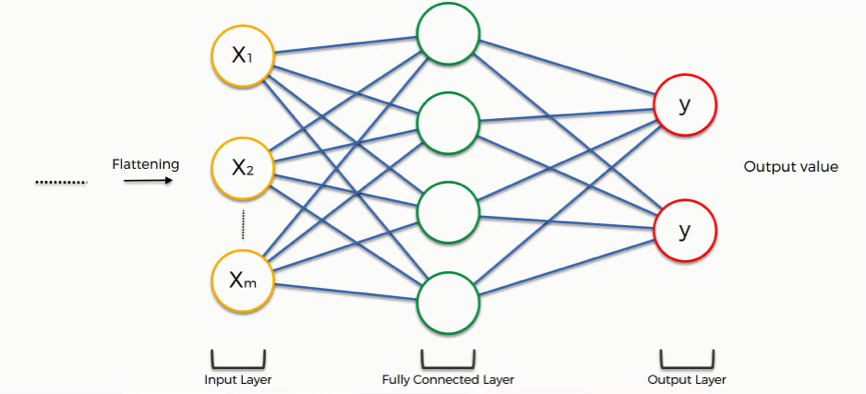
\includegraphics[scale=0.9]{figures/ffcexample}
    \captionsource{Simple neural network example}{https://www.superdatascience.com/blogs/convolutional-neural-networks-cnn-step-4-full-connection}
    \label{Simple neural network example}
\end{figure}

Figure \ref{Simple neural network example} visualizes how a simple fully connected neural network might look. The flattening refers to formatting the input features as a one-dimensional array to match the input layer size. This type of neural network is called fully connected, since each neuron is connected to every neuron in the next layer. The output layer represents the final binary classification step, where the two neurons stand for each of the two total categories this network is designed to identify.

Neuron connections have assigned weights. When the neural network model receives input, it is passed through the layers and gets multiplied by the weights. Assume an input neuron with value $x1$ is passed to a neuron in the next layer. The value of the neuron in the next layer will then be $w1(x1) + b1$, where $w1$ is the weight between the nodes and $b1$ is the bias term used to improve models flexibility. One might have noticed that the formula for passing data from one neurn to the other is a simple linear function. After the passing is done and the output layer is reached, the result in the output layer is some altered numerical representation of the input that can, depending on the goal, be interpreted as some prediction. For example, by applying a Softmax function on the output of the model, the result of each neuron would be between 0 and 1, and could be treated as the probabilities. This is a common way to do classification tasks. 

\begin{figure}[H]
    \centering
    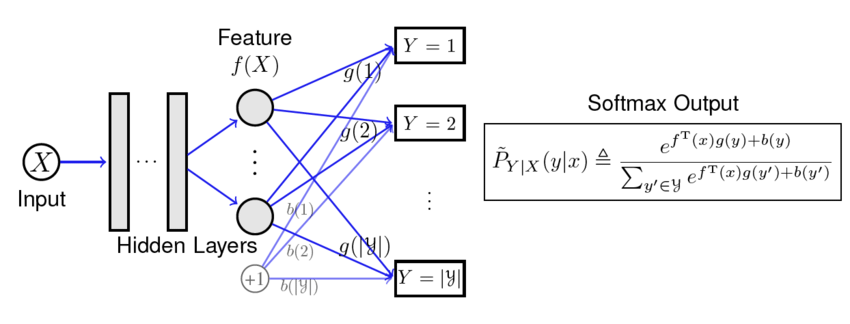
\includegraphics[scale=0.6]{figures/classificationExample}
    \caption{Classification example}
    \label{Classification example}
\end{figure}

Figure \ref{Classification example} shows another example of a classification network. This network has multiple hidden layers and an output layer with multiple classes from the set $Y$. To output the probabilities of an item being in each of the classes, the values from the output neurons are passed through the $softmax$ function.

Neurons also require an activation function to introduce non-linearity into the model. Without non-linearity, the multiplication of weights from each layer would result in a function that can be represented as a single linear transformation, defeating the purpose of having multiple layers in the architecture. A commonly used activation function is ReLU $max(0,x)$.

To teach the model, the weights of the neural network can be adjusted depending on the accuracy of the predictions by methods called back-propagation and gradient descend. Back-propagation calculates the impact of each weight on the total error using derivation. The error is calculated using a loss function such as negative log likelihood \[\text{NLL} = - \sum_{i=1}^{N} \sum_{j=1}^{C} y_{ij} \log(\hat{y}_{ij})\], where $N$ is the number of items, $C$ is the number of classes, $y_{ij}$ is $0$ or $1$ depending on whether class $j$ is correct for item $i$ and $\hat{y}_{ij}$ is the predicted class. Then, the gradient descend method is used to adjust the weights and potentialy lower the error in the next iteration. This process can be repeated multiple times, until the model can make predictions well enough. The process is fittingly called training. An important thing to keep in mind is that a trained model needs to be tested on unseen data since it can memorize all the data it was trained on. Overfitting is a term describing a model that learns the patterns of the training dataset near perfectly without being able to keep the same performance when given unseen data. In machine learning, one is interested in generalization, the model needs to find patterns that are common for all the relevant data it can encounter.

One epoch is described as one iteration of training where the model has gone through all the training data once. The number of epochs or how long the model must be trained depends heavily on the parameters and how complex the patterns are. Training can be stopped after a set number of epochs, if the information loss is nearing zero or when the loss plateaued indicating that the model cannot improve.

\section{Graphs}

The following gives a short introduction to what a graph is and the graph terminology used in this work.

A graph $G$ is a pair $(V,E)$, where $V$ is a set of vertices and $E$ is a set of edges between the vertices $E \subseteq \{(v,u) |  v,u \in V\}$ \cite{graphdef}. Two vertices with an edge between them are adjacent or connected. In an undirected graph an edge implies that the connection is bidirectional, meaning $(v,u)$ and $(u,v)$ are equivalent. Figure \ref{The difference between a directed and an undirected graph} demonstrates the difference between an undirected graph (right) and a directed graph (right).

\begin{figure}[H]
    \centering
    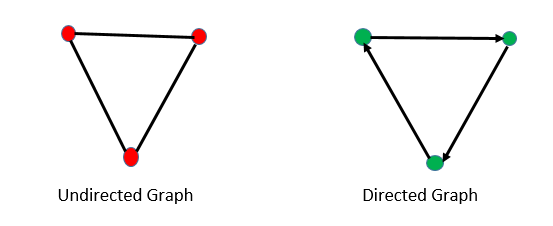
\includegraphics[scale=0.7]{figures/graph-theory}
    \captionsource{The difference between a directed and an undirected graph}{https://byjus.com/maths/graph-theory/}
    \label{The difference between a directed and an undirected graph}
\end{figure}

For graphs with weighted edges, let $W()$ be a weight function on the edges such that $W(e) \rightarrow \mathbb{Q}^+$ 

In this work we convert graphs to their line graph representation. The line graph is a complement of the original graph that turns each edge to a vertex and connects the vertices if they shared a vertex in the original graph. A simple example of a graph and its line graph can be seen in figure \ref{Line graph figure}.

\begin{figure}[H]
    \centering
    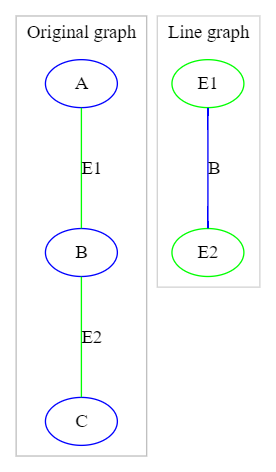
\includegraphics[scale=0.3]{figures/LineGraphExample}
    \caption{Original graph (left) and its line graph (right)}
    \label{Line graph figure}
\end{figure}

Note that the line graph willl always have the number of nodes equal to the number of edges in the original graph while, the number of edges in the line graph can vary and can be higher than the number of the original nodes.

In general, for graphs we use following notations: 
$$nodes/vertices: v \in V,$$
$$edges: e_{v,w} \in E | v, w \in V$$
$$neighbourhoods: N(v) \subseteq \{w, (v,w) \in E\}.$$ 

\section{Graph Neural Networks}
\label{sec:graphneuralnetworks}
Graph Neural Network (\gls{gnn}) is a relatively young subclass of neural networks designed specifically for solving graph related problems, and has been a growing topic of research in the last couple of years. \gls{gnn}s in general can be used for three purposes: graph prediction, node prediction and edge prediction. Graph prediction can be used to find graphs with desired properties, for example, to determine if a graph has cycles in it. Similarly, node and edge prediction is applicable to classification problems, such as identifying nodes and edges that are part of a cycle.

The application of graph prediction can be seen in bioinformatics. Ramachandran et al.\ have used graph convolutional network to predict how different proteins interact with each other \cite{ramachandran2019protein}. Node-level prediction has found application in traffic forecasting \cite{Yu2018}. Edge or link prediction models can be seen in the context of social networks with applications such as friends recommendation \cite{ADAMIC2003211}. Another popular field for \gls{gnn} research is Combinatorial Optimization (\gls{co}), which leads us to the well known problems such as the Maximum Weighted Matching (\gls{mwm}) and Maximal Independent Set (\gls{mis}).

Brusca et al.\ \cite{brusca2023maximum} showed a self-training \gls{gnn} for \gls{mis}. 

Schuetz et al.\ made an unsupervised \gls{gnn} \cite{Schuetz2022} for solving \gls{mis} and Angelini and Ricci-Tersenghi \cite{Angelini2022} compared its performance to greedy algorithms and reported some problems with \gls{gnn}s performance.

The reason \gls{mis} solving is mentioned is because the problem is to some degree related to \gls{mwm}, as algorithmic problems often are. There are concrete examples in the Methodology and Data chapter. \gls{mis} is also more often a subject for research, while research on \gls{mwm} is not that common. There are, however, some examples such as Wu and Li trying to solve \gls{mwm} using deep reinforcement learning \cite{WU2022400}. In this work they reported that their model outperforms state-of-the-art algorithms.

\gls{gnn}s are based on the same concepts as simple neural networks, but with some modifications to better suit graph, node and edge recognition problems. A simple \gls{gnn} can use a fully connected layer on each node and edge, as well as on the whole graph at once to generate a new numericatal representation for each element called embedding. In the following figure \ref{GNN example} one can see a simple overview of how the graph's information is passed from one layer to another, where $V$ denotes nodes, $E$ edges, $U$ graph-level features and update function is a neural network layer.

\begin{figure}[H]
    \centering
    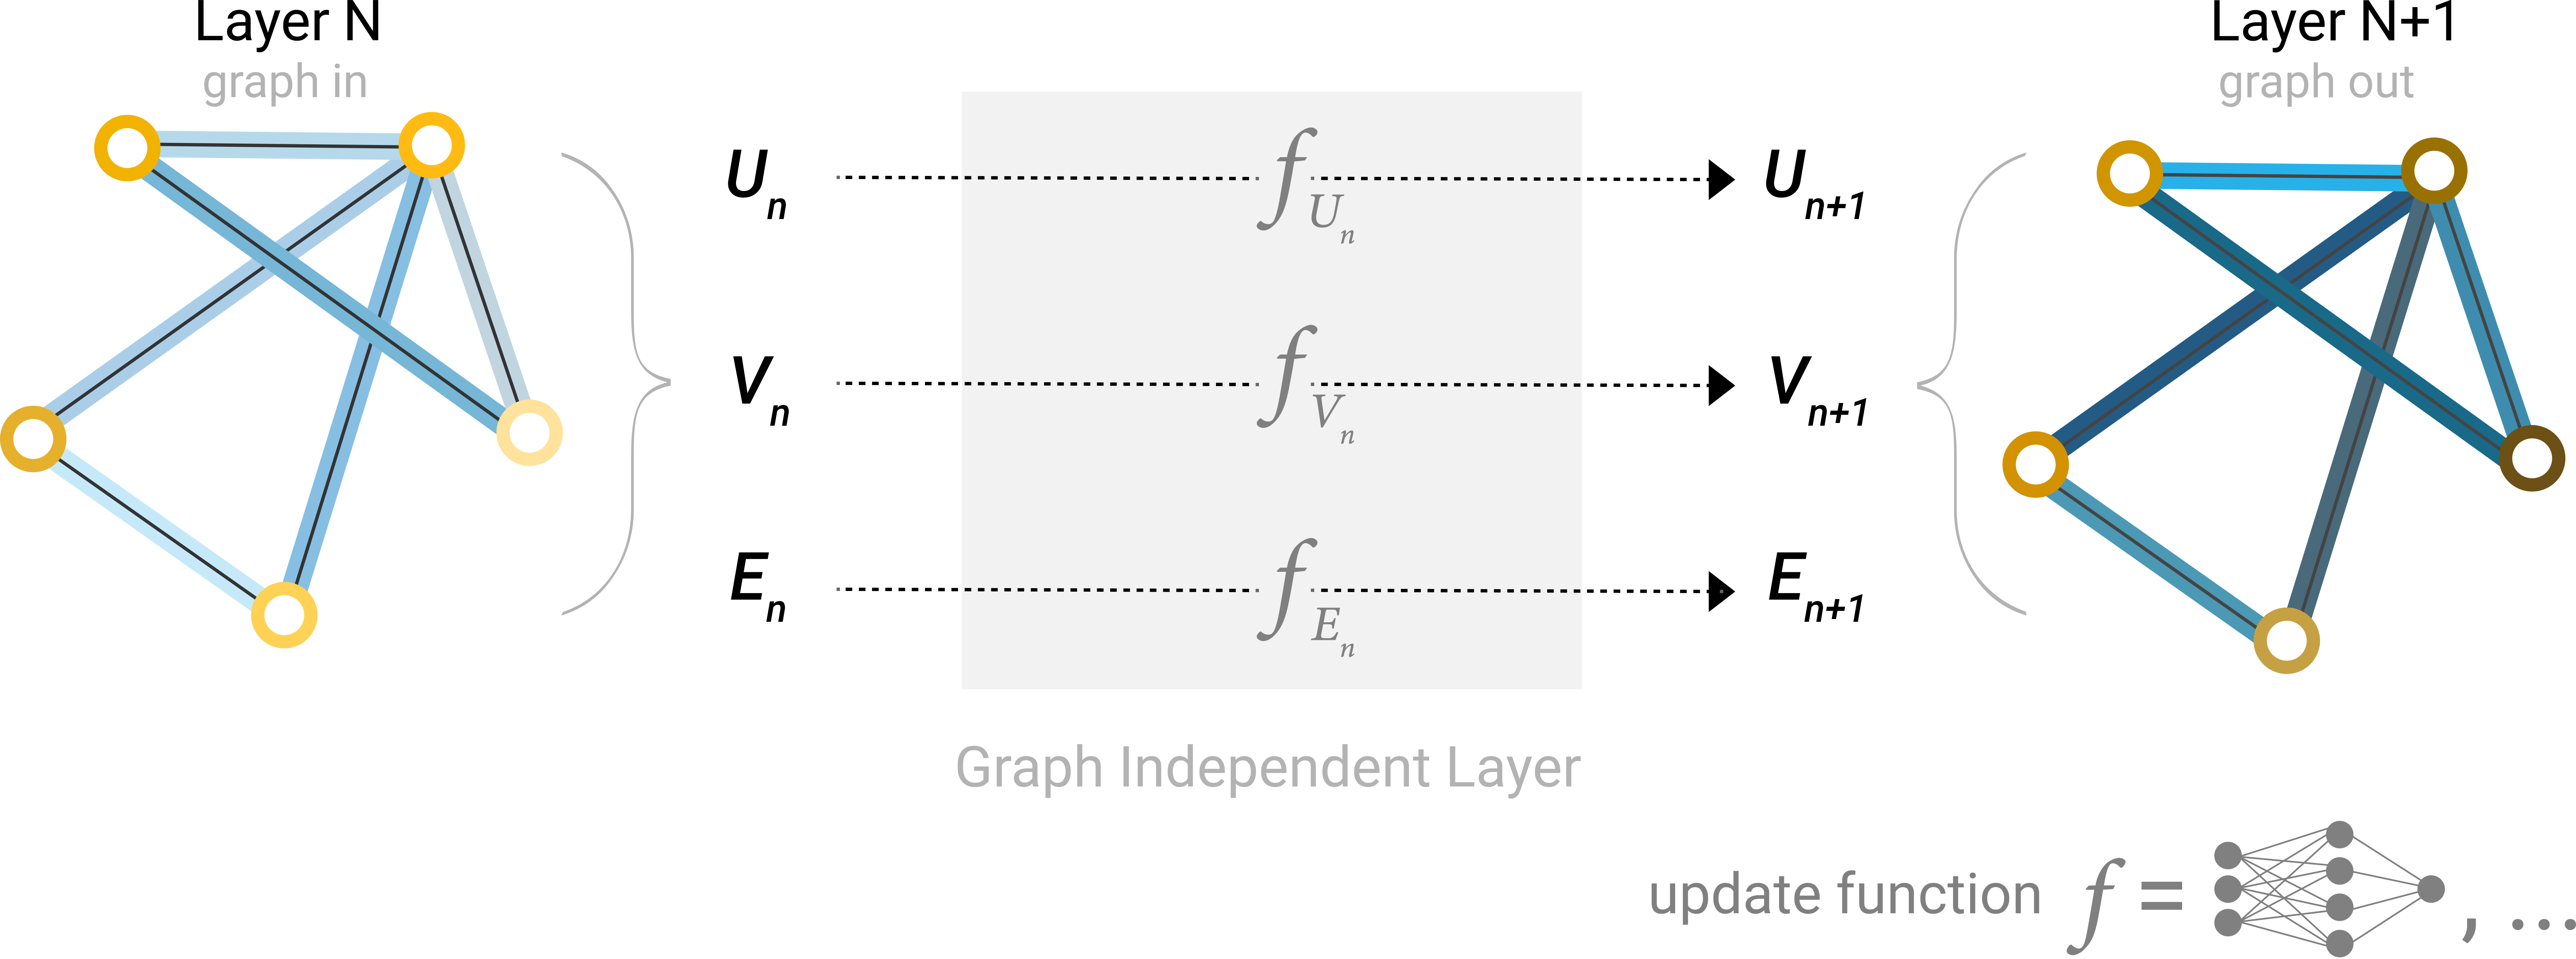
\includegraphics[scale=0.8]{figures/gnnintro}
    \captionsource{GNN example}{https://distill.pub/2021/gnn-intro/}
    \label{GNN example}
\end{figure}

For a simple node classification example, assume a graph with some nodes, where each node has two numerical features $f1$ and $f2$. Assume a \gls{gnn} that uses a simple fully connected network, where the input layer has two neurons, the middle layer has five and the output layer has two. For each node, the input layer reads the two features. Values of these features are then multiplied by the weights between each input neuron and each neuron in the next layer. One can express it as a matrix multiplication: 
$$
\begin{pmatrix}
f1 & f2 
\end{pmatrix}	
\times
\begin{pmatrix}
w11 & w12 & w13 & w14 & w15 \\
w21 & w22 & w23 & w24 & w25
\end{pmatrix}	
=
\begin{pmatrix}
n1 & n2 & n3 & n4 & n5 \\
\end{pmatrix}	
$$

Where the $f1, f2$ are node features and $w11$ to $w15$ are the five weights between the $f1$ input neuron and all the neurons in the next layers.

The information is then similarly passed from the middle layer to the output layer. The initial values of the node features have now been changed by the weights between the neurons, resulting in two output features. The \gls{gnn} has now produced an embedding for each node. Yet, the embeddings by themselves are not enough. In this example, the \gls{gnn} does not utilize the structure of the graph and the embedding of each node is not affected by its neighbours. 

If one wants to classify the nodes based on the node features only, then it can be done by using a standard neural network. However, for graphs, one is interested not only in the isolated node features, but in the nodes' relation to their neighbours. Additionally, graphs are not guaranteed to have any features for nodes and edges. 

What if one wants to use edges for classification of the nodes? In that case \gls{gnn} can use a pooling method. Pooling uses an aggregation function such as summation to sum together all the edge embeddings that a node has, and produce a new embedding. Alternatively, one can use neighbouring nodes for the same purpose, which leads to the specific type of \gls{gnn}s.

\gls{gcn} is one of the subclasses of \gls{gnn}s with some resemblance to the \gls{cnn}s used in image recognition. \gls{gcn} uses message passing to make use of the graphs' structure. For nodes, message passing gathers neighbouring node embeddings, aggregates the embeddings and then passes them through the network. The following figure \ref{Message passing example} shows how features from the neighbouring nodes are aggregated and passed to the next layer.

\begin{figure}[H]   
    \centering
    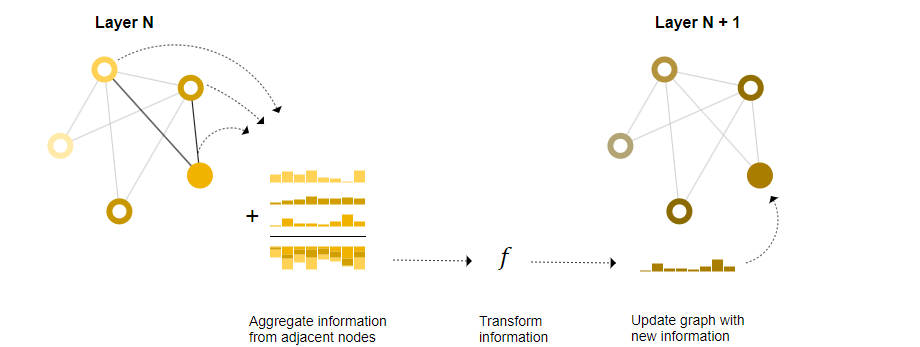
\includegraphics[scale=0.7]{figures/messagepassing}
    \captionsource{Message passing example}{https://distill.pub/2021/gnn-intro/}
    \label{Message passing example}
\end{figure}

Adding more layers increases the depth of the neighbourhood used. Meaning if a model has two layers, when passing through the second layer the embeddings of the neighbours are already an aggregation of its neighbours. This allows the \gls{gnn}s to utilize graph structure in a way that other neural networks cannot.

\begin{figure}[H]
    \centering
    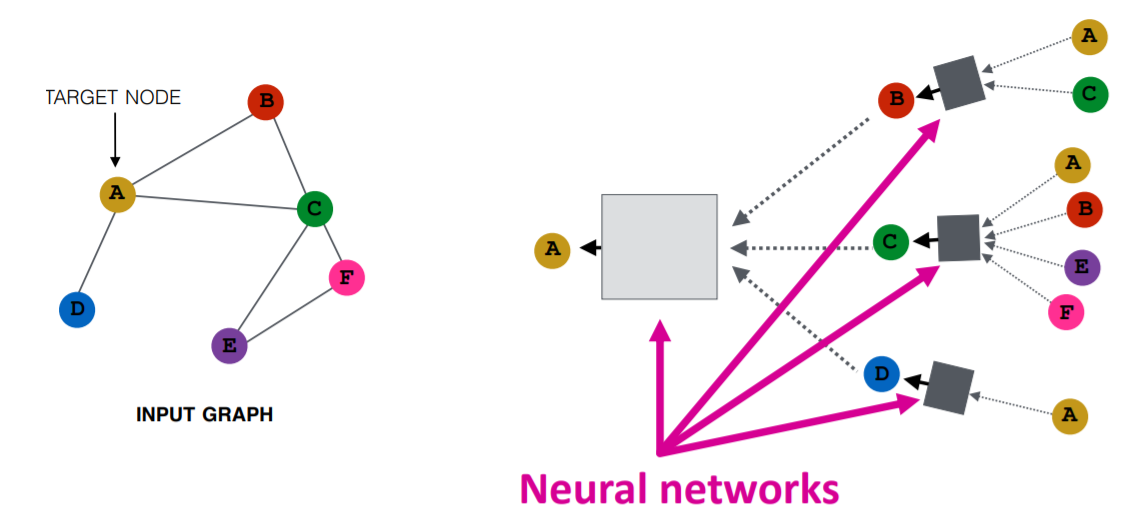
\includegraphics[scale=0.4]{figures/GNNExample}
    \captionsource{GCN example}{https://www.datacamp.com/tutorial/comprehensive-introduction-graph-neural-networks-gnns-tutorial}
    \label{GCN example}
\end{figure}

Figure \ref{GCN example} shows how two graph convolution layers affect a single node A.

\section{Implementation, training and hyperparameters}
\label{sec:implementation}

We have now gone through how \gls{gnn}s work from a high level view. However, it remains to create a \gls{gnn} as well as to train it. In this work we use \gls{pyg} library \cite{pytorchlib} that provides both the impementation for the various \gls{gnn} architectures and the tools to train the models. 

\subsection{Implementation}

The code snippet below \ref{Creating GCN with Pytorch} demonstrates how to create a simple \gls{gcn} by inheriting the base class $torch.nn.Module$. 

\begin{lstlisting}[caption={Creating GCN with Pytorch}, label={Creating GCN with Pytorch}, language=Python]
import torch
import torch.nn.functional as F
from torch_geometric.nn import GCNConv, Linear

class MyGCN(torch.nn.Module):
    def __init__(self):
        super().__init__()
        self.conv1 = GCNConv(1, 64) # 1 feature per each node
        self.conv2 = GCNConv(64, 64)
        self.lin = Linear(64, 2) # 2 classes 

    def forward(self, graph):        
        x, edge_index, edge_weight = graph.x, graph.edge_index, graph.edge_weight
        
        x = self.conv1(x, edge_index, edge_weight)
        x = F.relu(x)
        
        x = self.conv2(x, edge_index, edge_weight)
        x = F.relu(x)
        
        x = self.lin(x)
        return F.log_softmax(x, dim=1)    
\end{lstlisting}

A module in Pytorch can be a part of a larger network or a whole network in this case. One can add layers to the network by assigning other modules within the initializer function. Here, we add three layers. The first layer, $self.conv1 = GCNConv(1,64)$ is the input layer with one input neuron and 64 output neurons. This layer will require all nodes to have exactly one feature. To connect the $conv1$ layer to the second one, $conv2$, they must have a matching number of output and input neurons (64 in this example) respectively. The output module $self.lin = Linear(64, 2)$, is a simple fully connected layer that maps output neurons from the $conv2$ to the two neurons representing the two possible predictions. For example, whether a node should or should not be in the solution. In the $forward$ function, one has to define the order in which the information will flow through the network. First, one has to read the input from the graph. The $x$ represents the array of node features. In this case, the array is of size one. The $edge\_index$ and $edge\_weight$ represent the edges and their weights respectively. The $torch.nn.functional$ library provides the tool for mathematical operations and is used to apply the $F.relu$ activation function to the neurons as well as $F.log\_softmax$ to the output. The $relu = max(0,x)$ activation function serves the purpose of adding non-linearity to the network, enabling it to form complex patterns. The $F.log\_softmax$ function maps the output values into the desired range for measuring the error. Which function is used depends on how the error is calculated.

\subsection{Training}

To train the model described above, the following procedure can be done, demonstrated in the next listing \ref{Training GCN with Pytorch}. 

\begin{lstlisting}[caption={Training GCN with Pytorch}, label={Training GCN with Pytorch}, language=Python]
import torch
import torch.nn.functional as F
from torch_geometric.loader import DataLoader

device = torch.device('cuda' if torch.cuda.is_available() else 'cpu')
loader = DataLoader(dataset, shuffle=True)
optimizer = torch.optim.Adam(list(model.parameters()), lr=0.0005)

for epoch in range(100):        
    for graph in loader:
        optimizer.zero_grad()
        
        graph = graph.to(device)
        out = model(graph).to(device)   
            
        loss = F.nll_loss(out, graph.y)
        loss.backward()

        optimizer.step()
\end{lstlisting}

First, the $DataLoader$ and optimizer are initialized. The $DataLoader$ is responsible for managing and preproccessing the data. In this case, it only shuffles the dataset items randomly. The optimizer is used to preform the gradient descent on the models weights. Adam \cite{ADAMIC2003211} is a commonly used optimizer that has several parameters such as learning rate (lr) that affect the training process and how the weights are updated. These parameters in the context of the model are called the model's hyperparameters. With dataloader and optimizer ready, the main training loop starts. For each epoch or iteration, we retrieve the next batch of data from the $dataloader$. Before updating weights, $optimizer.zero\_grad()$ is called to make sure that the optimizer's gradients are reset. Then we pass the graph to the GPU device if possible to speed up the calculations. The graph is then passed through the model with the output mapped using $log\_softmax$ within the model's forward function. The $log\_softmax$ mapping produces the logarithmic probabilities required by the $nll\_loss$ function to compute the error or information loss made from the model's output in regard to the correct answers contained in $graph.y$. The error is then propagated backward by calling $loss.backward()$, determining the impact each weight made and then $optimizer.step()$ updates the weights based on the current hyperparameters.

\subsection{Hyperparameters}

The term “hyperparameter” refers to the parameters used to adjust the training process and the architecture of the network, while “parameters” refer to the weights between neurons. In this work we test several hyperparameters that can be further split into categories.

The training and Adam optimizer related hyperparameters include:
\begin{itemize}
\item Epochs - the number of training iterations. The longer a model is trained the less errors it should make, given the sufficient complexity of the model.
\item Learning rate - by how much the weights of the model should be adjusted after each iteration. Small steps have a risk of a model getting stuck in a place where the changes do not improve the results, while a significantly different configuration of weights that gives better results might exist. Small steps also might require to train the model for longer to reach the desired level of performance. Too large learning rates have a risk of overstepping the better weight configurations.
\item Mini-Batching size - how many graphs are passed through the network before next weight adjustment. Passing data in batches can help to smooth the learning curve and reduce the risk of overfitting.
\item Class weights - how much should the model focus on a given class. Class weights can help with data imbalance where one class occurs more often than others. For example if 99\% of objects belong to one class, but the model needs to focus on finding the other 1\%. In our case the classes for the edges are: 
	\begin{itemize}
	\item 0 = is NOT in the solution.
	\item 1 = is in the solution.
	\end{itemize}	
\item Weight decay - used to keep \gls{gnn} weight values relatively small and decrease chances of the overfitting. 
\end{itemize}

The architecture related hyperparameters affect the capability of the network to learn complex patterns. 
\begin{itemize}
\item Network width - neurons in the layers.
\item Network depth - amount of layers. In case of \gls{gcn}s, the depth of the network also defines the radius of the aggregated node neighbourhood. 
\end{itemize}

The aggregation of neighbours is the key feature of the \gls{gnn}s and there are multiple functions that can be used.
\gls{gnn} specific hyperparameters:
\begin{itemize}
\item Aggregation function - the features of the neighbouring nodes can be aggregated by using different methods, including summation, maximum, minimum, multiplication and division.
\end{itemize}

Additionally one can experiment with adding extra features to the nodes during preprocessing or augmenting data. Examples of such features for the weighted graph are: 
\begin{itemize}
\item Degree - how many neighbours a node has
\item Sum of the weights. 
\end{itemize}
Such features can help the model to find new patterns.

The hyperparameter search helps to fit the model specifically for the desired task. In our case the model needs to learn how to solve Maximum Weighted Matching (MWM) on graphs.

\section{Maximum Weighted Matching and Combinatorial Optimization}

Combinatorial Optimization (CO) is a field of study that covers problems that require finding a subset or a combination of some set of elements that fulfills certain requirements. An example of such a problem would be Maximum Weighted Matching \gls{mwm} and Maximum Independent Set \gls{mis}. 

The \gls{mwm} problem asks to find a subset of edges in a weighted graph, such that the sum of weights is maximized, and each vertex appears only in one edge of that subset. More formally, given an undirected graph $G$ with a set of vertices $V$ and a set of weighted edges $E$, maximize total weight for set $S \subseteq E$, such that none of the edges in $S$ share vertices. In this work, the edges that are selected to be in the solution set will sometimes be referred to as “picked” and the ones that are not in the set “dropped”.

The \gls{mwm} problem is relatively simple compared to many others. It belongs to the field of \gls{co} and there are optimal algorithms for it that run in $O(|V|^{2}|E|)$ time, such as the blossom algorithm \cite{blossom}. Blossom algorithm is based on the blossom method for finding augmenting paths and the primal-dual method for finding a matching of maximum weight, both due to Jack Edmonds \cite{blossom}.

Optimal algorithms, however, can still be rather slow when working with large datasets, and in some cases an approximation algorithm may be more suitable as a solution if the exact answer is not critically important for the \gls{mwm} problem. The most simple example is a greedy algorithm that sorts all the edges by their weight and selects them in descending order. This is neither the only nor the best approximation algorithm, but rather a fast and simple one.

\begin{algorithm}
\caption{Greedy algorithm for Maximum Weighted Matching}\label{alg:cap}

\begin{algorithmic}
\State G(V,E)
\State $S = \emptyset$
\State $sortedE = descendingSort(E)$
\While{$sortedE \neq \emptyset$}
\State $e$ = first element in sortedE
\If{$e$ not adjacent to any edge in S}
  \State add e to $S$
  \State remove $e$ from sortedE
\EndIf
\EndWhile
\end{algorithmic}
\end{algorithm}

The running time of the Greedy algorithm is bound by the sorting, since the While loop iterates through the edges once and runs in $O(|E|)$. The fastest sorting runs in $O(|E| log(|E|))$.

To put \gls{mwm} in context, real world applications of matching algorithms can be found in scheduling problems such as transportation cost minimization \cite{mwmExample}, but are also often used as a part of larger algorithms.

Another problem that will be slightly touched is the Maximal Independent Set (\gls{mis}). \gls{mis} asks to find a subset of nodes such that no two nodes have an edge between them, and the total number of nodes is as large as possible. There is a similar problem \gls{mwis} which asks us to find an independent set in graph with weighted nodes that gives the largest total weight sum. \gls{mwis} is partially relevant as we use line graph transformation that essentially turns the original \gls{mwm} problem into \gls{mwis}.
